\section{Data Extraction and Analysis}

In order to extract content from multiple web pages, a web crawler will need to be created using the Python programming language. The group plans on using Scrapy, a Python library which will handle the "`visiting"' of websites, when provided with a sufficient list of hosts. Scrapy crawls through each directory within the host (as defined by the site's \textsl{robots.txt} file). After visiting a URL, the content will be extracted and analysed using the information retrieval methods available in the Python Natural Language Toolkit (NLTK) library.

\begin{figure}
  \centering
  \begin{minipage}{7cm}
    \centering
    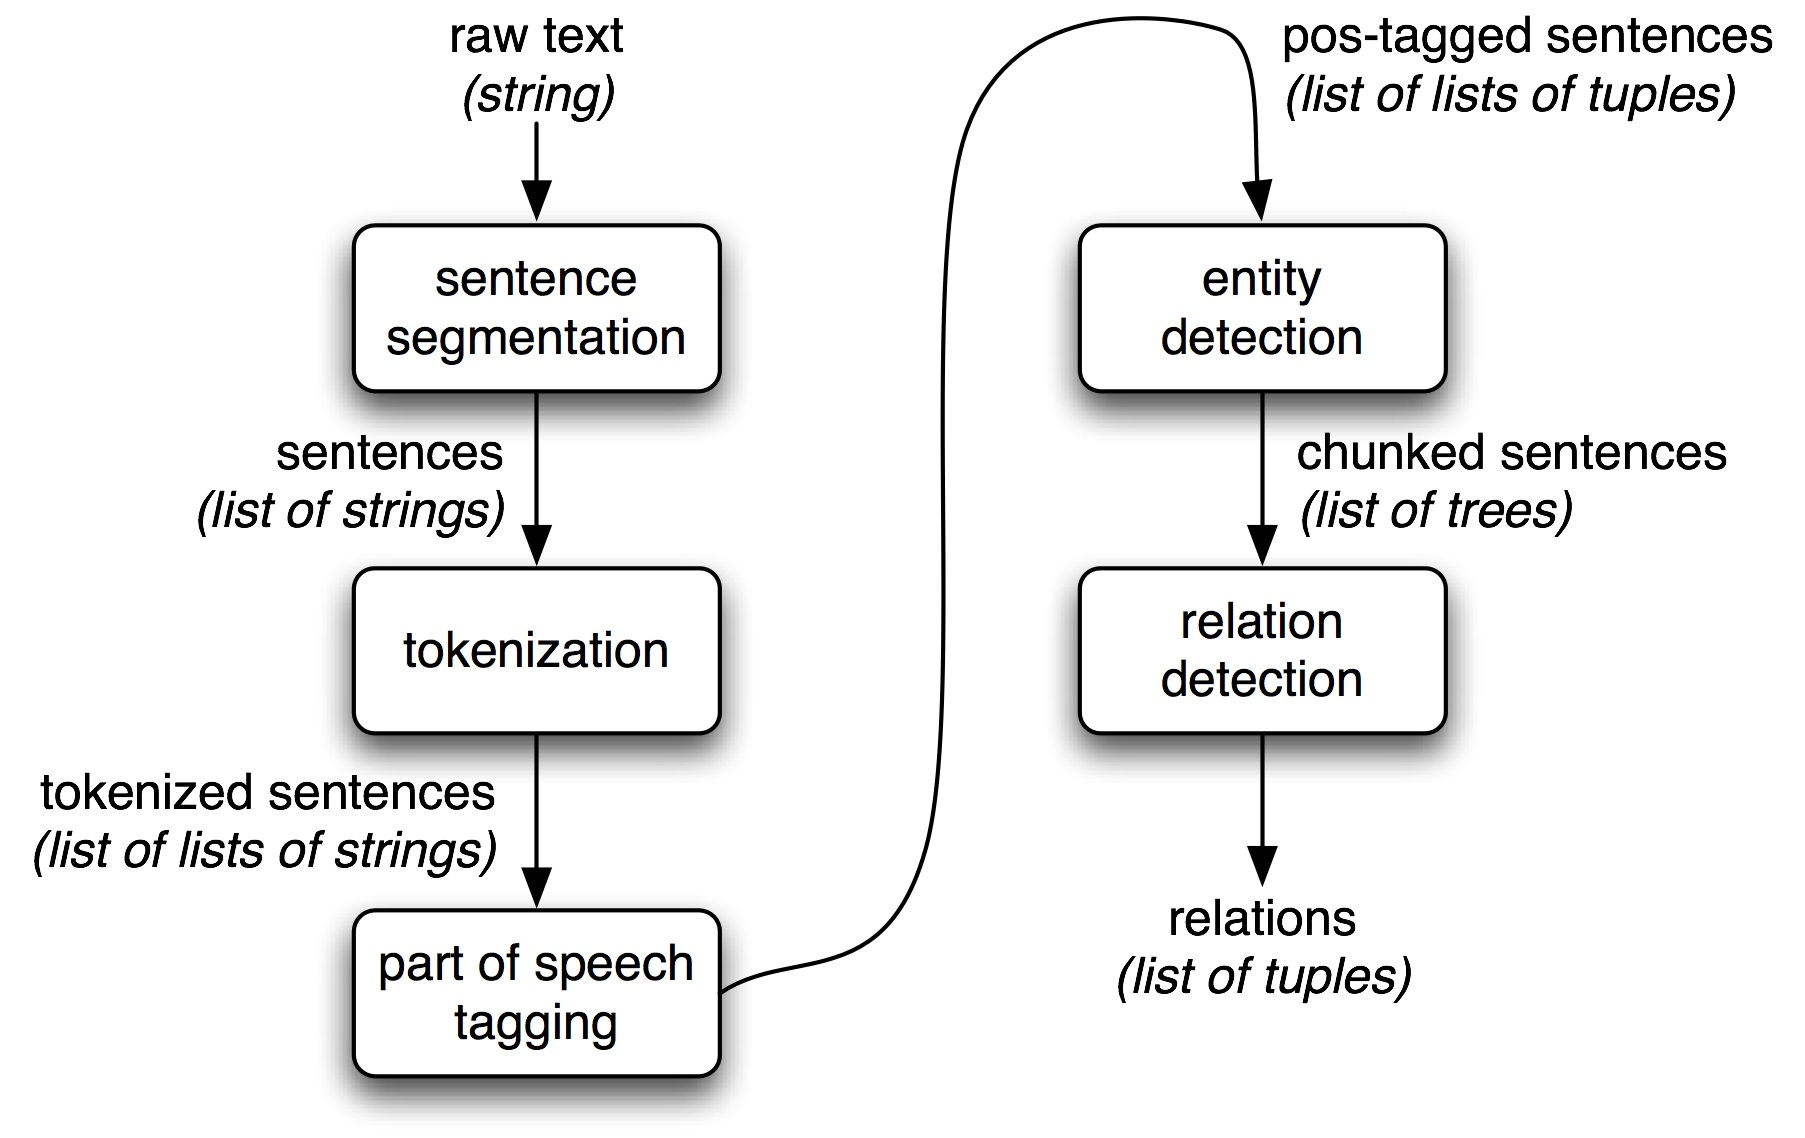
\includegraphics[width=7cm]{inc/ie-architecture.jpg}
    \caption{Python Natural Language Tookit Information Retrieval Flow Diagram}
    \label{fig:information_retrieval}
  \end{minipage}
\end{figure}

Many websites implement measures to prevent web crawlers from crawling due to the number of requests made as they utilise their server resources. Quite often, this results in the crawler being banned. However, the group can take the following measures to prevent this:

\begin{itemize}
  \item Disabling cookies may prevent getting banned, but only if it’s the method used by the website to detect crawlers
  \item Using Google cached pages instead of visiting the websites directly
  \item Using different IP addresses by rotating from a list when making a request to the same host
  \item Setting a delay between requests
\end{itemize}
